\section{Minimum network flow problem}

The network flow problem involves efficiently distributing a particular product from a set of sources to a set of users in order to optimize a predefined objective function.
    \begin{definition}
    A network is a directed and connected graph $G = (V,A)$ with a source $s \in V$ and a sink $t \in V$, with $s \neq t$, and a capacity $k_{ij} \geq 0$ for each arc 
    $(i,j) \in A$. 

    A \emph{feasible flow} $x$ from $s$ to $t$ is a vector $x \in \mathbb{R}^m$ with a component $x_{ij}$ for each arc $(i,j) \in A$ satisfying the capacity constraints:
    \[0 \leq x_{ij} \leq k_{ij} \:\:\:\:\:\: \forall (i,j) \in A\]
    and the flow balance constraints at each intermediate node $u \in V (u \neq s,t)$: 
    \[\sum_{(i,u)\in \delta^{-}(u)}x_{iu}=\sum_{(u,j)\in \delta^{+}(u)}x_{uj} \:\:\:\:\:\: \forall u \in N-\{s,t\}\]

    The \emph{value of flow} $x$ is:
    \[\varphi = \sum_{(s,j) \in \delta^{+}(s)} x_{sj}\]

    Given a network and a feasible flow $x$, an arc $(i,j) \in A$ is \emph{saturated} if $x_{ij} = k_{ij}$. 

    Given a network and a feasible flow $x$, an arc $(i,j) \in A$ is \emph{empty} if $x_{ij} = 0$. 
\end{definition}
In the network flow problem, we are given a network $G = (V,A)$ with integer capacities $k_{ij}$ for each arc $(i,j) \in A$, and two designated nodes $s,t \in V$. 
The goal is to determine a feasible flow from $s$ to $t$ with the maximum value.

In cases where there are multiple sources and sinks with a single type of product, dummy nodes $s^{*}$ and $t^{*}$ can be introduced. 
The linear programming model for this problem aims to maximize $\max \varphi$, subject to the following constraints:
\[\sum_{(u,j)\in \delta^{+}(u)}x_{uj}-\sum_{(i,u)\in \delta^{-}(u)}x_{iu}=
\begin{cases}
    \varphi \:\:\:\:\:\:\:\:\: u=s    \\
    -\varphi \:\:\:\:\:\: u=t   \\
    0 \:\:\:\:\:\:\:\:\:\: \textnormal{otherwise}
\end{cases}\]
Here, $\varphi$ represents the value of the feasible flow $x$, $0 \leq x_{ij} \leq k_{ij}$ with $\varphi,x_{ij} \in \mathbb{R}$, and $(i,j) \in A$.
\begin{definition}
    A \emph{cut separating $s$ from $t$} is $\delta(S)$ of $G$ with $s \in S \subset V$ and $t \in V-S$. There are $2^{n-2}$ cuts separating $s$ from $t$, where 
    $n=\left\lvert V \right\rvert $.

    The \emph{capacity of the cut} $\delta(S)$ induced by $S$ is equal to: 
    \[k(S)=\sum_{(i,j)\in \delta^{+}(S)}k_{ij}\]

    Given a feasible flow $x$ from $s$ to $t$ and a cut $\delta(S)$ separating $s$ from $t$, the \emph{value of the feasible flow x through the cut $\delta(S)$} is: 
    \[\varphi(S)=\sum_{(i,j)\in \delta^{+}(S)}x_{ij} - \sum_{(i,j)\in \delta^{-}(S)}x_{ij}\]
\end{definition}
With this notation, the value of the flow $x$ is represented as $\varphi = \varphi(\{s\})$. 
\begin{property}
    Given a feasible flow $x$ from $s$ to $t$, for each cut $\delta(S)$ separating $s$ from $t$, we have $\varphi(S)=\varphi(\{s\})$.
\end{property}
\begin{property}
    For every feasible flow $x$ from $s$ to $t$ and every cut $\delta(S)$, with $S \subseteq V$, separating $s$ from $t$, we have $\varphi(S) \leq k(S)$:
    \[\varphi(S) \leq k(S)\]
    This expression signifies that the flow's value is either less than or equal to the capacity of the cut.
\end{property}
\begin{proof}
    According to the definition of the flow value through the cut $\delta(S)$, we express it as:
    \[\varphi(S)=\sum_{(i,j) \in \delta^{+}(S)}x_{ij}-\sum_{(i,j) \in \delta^{-}(S)}x_{ij}\]
    Furthermore, considering that $0 \leq x_{ij } \leq k_{ij}$ for any edge $(i, j) \in A$, we can establish:
    \[\sum_{(i,j) \in \delta^{+}(S)}x_{ij}-\sum_{(i,j) \in \delta^{-}(S)}x_{ij} \leq \sum_{(i,j) \in \delta^{+}(S)}k_{ij}=k(S)\]
    Hence, it follows that $\varphi(S) \leq k(S)$.
\end{proof}
\begin{example}
    The value of the feasible flow $x$ passing through the cut $\delta(S)$  in the graph is illustrated below:
    \begin{figure}[H]
        \centering
        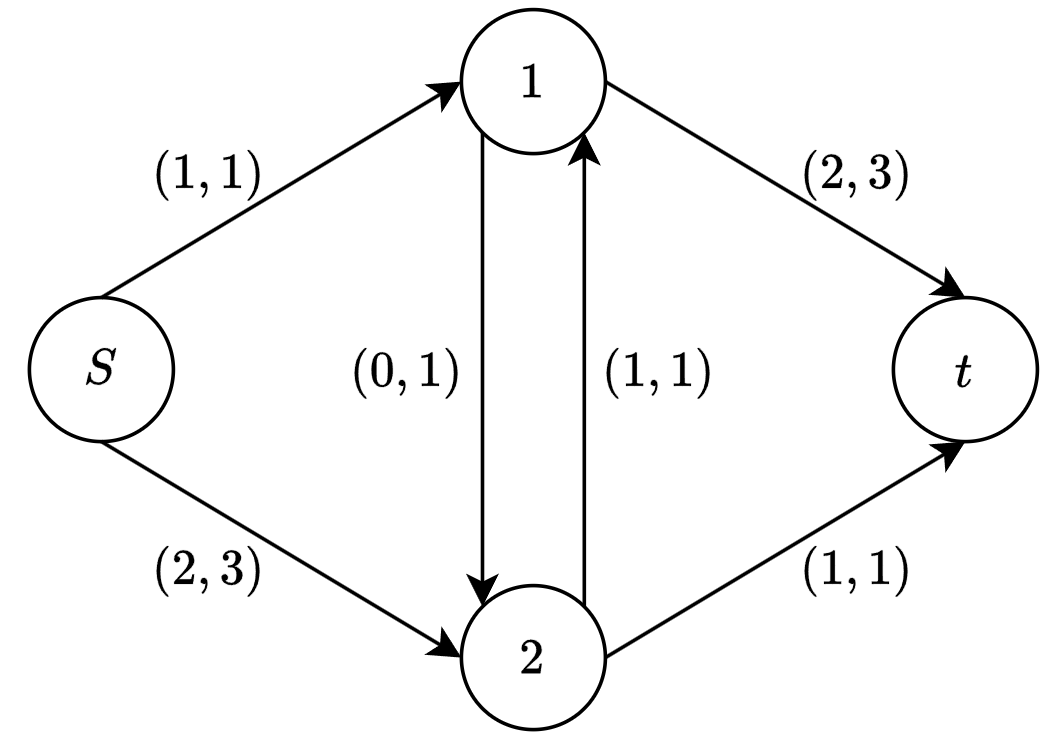
\includegraphics[width=0.25\linewidth]{images/flow.png}
    \end{figure}
    \[\varphi(\{s,1\})=2+0+2-1=3\]
    The remaining values are as follows: 
    \[\delta(\{s,1\})=\{(s, 2),(1,2),(1, t)\}\]
    \[k(S)=7\]
\end{example}
If $\varphi(S) = k(S)$ for a subset $S \subseteq V$ containing the source $s \in S$ and excluding the destination $t \notin S$, then the flow $x$ attains its maximum value, and the cut $\delta(S)$ represents the minimum capacity. 
The property $\varphi(S) \leq k(S)$ for any feasible flow $x$ and any cut $\delta(S)$ that separates $s$ from $t$ signifies a weak duality connection between two problems:
\begin{itemize}
    \item Determining a feasible flow of maximum value in a graph $G = (V, A)$ with integer capacities on the arcs and source-destination pair $s, t \in V$.
    \item Identifying a cut (one that separates $s$ from $t$) of minimum capacity in a graph $G = (V, A)$ with integer arc capacities and source-destination pair $s, t \in V$.
\end{itemize} 
The idea of the Ford-Fulkerson's algorithm to find network flows is as follows: start from a feasible flow $x$ and try to iteratively increase its value $\varphi$ by sending, at each iteration, an additional amount of product along an undirected path from $s$ to $t$ with a strictly positive residual capacity. 
If the arc $(i,j)$ is not saturated, we can increase $x_{ij}$. 
If $(i,j)$ is not empty, we can decrease $x_{ij}$ while respecting $0 \leq x_{ij} \leq k_{ij}$. 
\begin{definition}
    A path $P$ from $s$ to $t$ is an \emph{augmenting path} with respect to the current feasible flow $x$ if $x_{ij} <  k_{ij}$ for any
    forward arc $x_{ij}>0$ for any backward arc. 
\end{definition}
Given a feasible flow $x$ for $G=(V,A)$, we create the residual network denoted as $\overline{G}=(V,\overline{A})$ associated to $x$. 
This residual network encompasses all conceivable adjustments to the flow $x$: 
\begin{itemize}
    \item If $(i,j) \in A$ is not empty $(i,j) \in \overline{A}$ with $\overline{k}_{ij}=x_{ij}>0$.
    \item If $(i,j) \in A$ is not saturated $(i,j) \in \overline{A}$ with $\overline{k}_{ij}=k_{ij}-x_{ij}>0$
\end{itemize}
Here, $\overline{k}_{ij}$ is termed residual capacity. 
\begin{example}
    To determine the residual capacity of the graph depicted below, we follow this procedure:
    \begin{figure}[H]
        \centering
        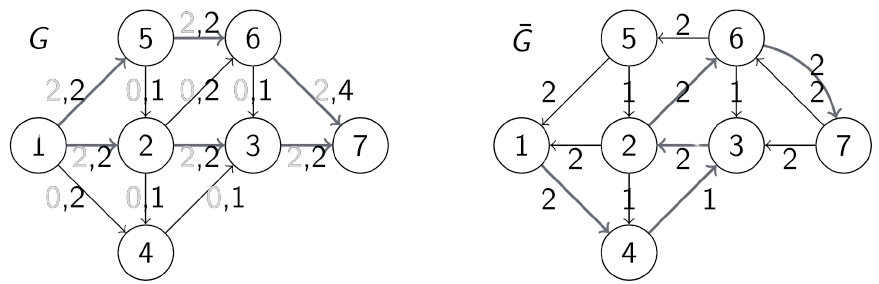
\includegraphics[width=0.75\linewidth]{images/residual1.png}
    \end{figure}
    Afterward, we update the flow and once more compute the residual capacity:
    \begin{figure}[H]
        \centering
        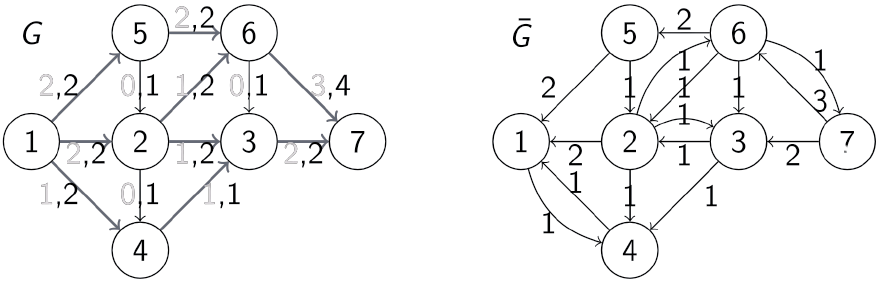
\includegraphics[width=0.75\linewidth]{images/residual2.png}
    \end{figure}
    This process is repeated:
    \begin{figure}[H]
        \centering
        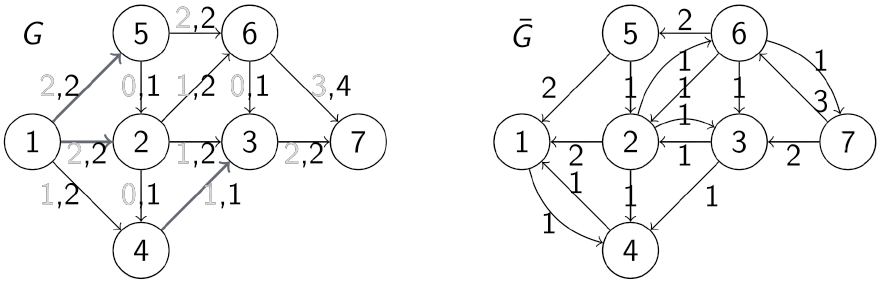
\includegraphics[width=0.75\linewidth]{images/residual3.png}
    \end{figure}
    However, since we are unable to identify additional paths, we conclude that the flow is now $\phi=5$.
\end{example}
\begin{proposition}
    Ford-Fulkerson's algorithm is exact. 
\end{proposition}
\begin{proof}
    A feasible flow denoted as $x$  achieves its maximum value if and only if the destination node $t$ cannot be reached from the source node $s$ in the residual network associated with flow $x$. 
    If an augmenting path exists, then flow $x$ is not optimal for achieving the maximum value.
    When $t$ is not reachable from $s$, it implies the presence of a cut in the residual network $\overline{G}$ such that $\delta^{+}_{\overline{G}}(S^{*})=\varnothing$. 
    By the definition of $\overline{G}$  every edge $(i,j) \in \delta^{+}_{G}(S^{*})$ is saturated, and every edge in $\delta^{-}_{G}(S^{*})$ is empty. 
    Consequently,
    \[\phi(S^{*})=\sum_{(i,j) \in \delta^{+}_{G}(S^{*})}{x_{ij}}-\sum_{(i,j) \in \delta^{-}_{G}(S^{*})}{x_{ij}}= \sum_{(i,j) \in \delta^{+}_{G}(S^{*})}{k_{ij}}=k(S^{*})\]
    According to weak duality, it follows that $\phi(S) < k(S)$ for all feasible flows $x$ and $\forall S \subset V$ with $s \in S$, $t \notin S$. 
    Therefore, the flow $x$ has maximum value and the cut induced by $S^{*}$ represents the minimum capacity.
\end{proof}
\begin{theorem}
    The value of a feasible flow of maximum value is equal to the capacity of a cut of minimum capacity.
\end{theorem}
The algorithm takes as its inputs a graph denoted as $G=(V,A)$ with non-zero capacities $k_{ij}>0$ for all edges $(i,j) \in A$, where $t \in N$. 
\begin{algorithm}[H]
    \caption{Ford-Fulkerson's algorithm}
        \begin{algorithmic}[1]
            \State $x \leftarrow 0$
            \State $\phi \leftarrow 0$
            \State $\textnormal{optimum} \leftarrow \textnormal{false}$
            \While {optimum = true}
                \State Build residual network $\overline{G}$ associated to $x$
                \State $P \leftarrow$ path from $s$ to $t$ in $\overline{G}$
                \If {$P$ is not defined}
                    \State optimum $\leftarrow$ true
                \Else
                    \State $\delta \leftarrow \min\{\overline{k}_{ij}|(i,j) \in P\}$
                    \State $\phi \leftarrow \phi + \delta$
                    \For {$(i,j) \in P$}
                        \If {$(i,j)$ is a forward arc}
                            \State $x_{ij} \leftarrow x_{ij}+\delta$
                        \Else 
                            \State $x_{ij} \leftarrow x_{ij}-\delta$
                        \EndIf
                    \EndFor
                \EndIf
            \EndWhile
        \end{algorithmic}
\end{algorithm}
The algorithm's total complexity is $O(m^2k_{max})$. 
The space complexity of the algorithm is $O(m\log{k_{max}})$. 
To render the algorithm polynomial, one can seek an augmenting path with the minimal number of arcs.

\subsection*{Minimum cost flow problem}
In the context of a network with unit costs denoted as $c_{ij}$ or each arc  $(i,j)$ and a specified value $\phi > 0$the objective is to find a feasible flow from source $s$ to destination $t$ with a value of $\phi$ while minimizing the total cost.
To address this problem, the approach involves initiating from a feasible flow $x$ with a value of $\phi$ and dispatching an additional quantity of goods within the residual network through cycles characterized by negative costs.

\subsection*{Assignment problem}
\begin{definition}
    Given an undirected bipartite graph $G=(V,E)$, a \emph{matching} $M \subseteq E$ is a subset of non-adjacent edges. 
\end{definition}
\begin{figure}[H]
    \centering
    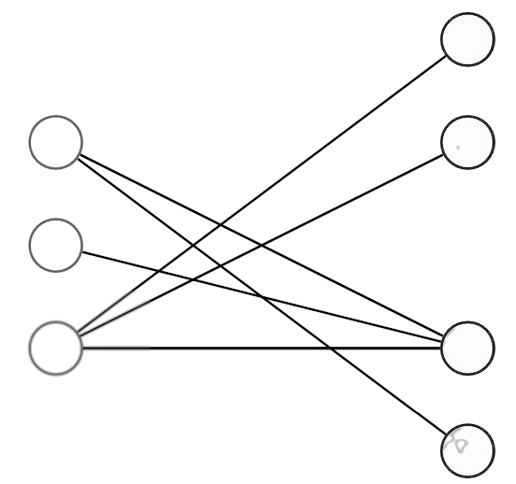
\includegraphics[width=0.2\linewidth]{images/matching.png}
\end{figure}
Given a bipartite graph $G=(V,E)$, determine a matching with a maximum number of edges. 
This problem can be reduced to the problem of finding a feasible flow of maximum value from $s$ to $t$ in the following network. 
There is a correspondence between the feasible flow of value $\varphi$ and the matching containing $\varphi$ edges. 